\documentclass[12pt,letterpaper]{article}
\usepackage{graphicx,textcomp}
\usepackage{natbib}
\usepackage{setspace}
\usepackage{fullpage}
\usepackage{color}
\usepackage[reqno]{amsmath}
\usepackage{amsthm}
\usepackage{fancyvrb}
\usepackage{amssymb,enumerate}
\usepackage[all]{xy}
\usepackage{endnotes}
\usepackage{lscape}
\newtheorem{com}{Comment}
\usepackage{float}
\usepackage{hyperref}
\newtheorem{lem} {Lemma}
\newtheorem{prop}{Proposition}
\newtheorem{thm}{Theorem}
\newtheorem{defn}{Definition}
\newtheorem{cor}{Corollary}
\newtheorem{obs}{Observation}
\usepackage[compact]{titlesec}
\usepackage{dcolumn}
\usepackage{tikz}
\usetikzlibrary{arrows}
\usepackage{multirow}
\usepackage{xcolor}
\newcolumntype{.}{D{.}{.}{-1}}
\newcolumntype{d}[1]{D{.}{.}{#1}}
\definecolor{light-gray}{gray}{0.65}
\usepackage{url}
\usepackage{listings}
\usepackage{color}
\usepackage{tabularx}


\definecolor{codegreen}{rgb}{0,0.6,0}
\definecolor{codegray}{rgb}{0.5,0.5,0.5}
\definecolor{codepurple}{rgb}{0.58,0,0.82}
\definecolor{backcolour}{rgb}{0.95,0.95,0.92}

\lstdefinestyle{mystyle}{
	backgroundcolor=\color{backcolour},   
	commentstyle=\color{codegreen},
	keywordstyle=\color{magenta},
	numberstyle=\tiny\color{codegray},
	stringstyle=\color{codepurple},
	basicstyle=\footnotesize,
	breakatwhitespace=false,         
	breaklines=true,                 
	captionpos=b,                    
	keepspaces=true,                 
	numbers=left,                    
	numbersep=5pt,                  
	showspaces=false,                
	showstringspaces=false,
	showtabs=false,                  
	tabsize=2
}
\lstset{style=mystyle}
\newcommand{\Sref}[1]{Section~\ref{#1}}
\newtheorem{hyp}{Hypothesis}

\title{Replication Project}
\date{Paper title: \\
	Movement versus Party: The Electoral Effects \\
	of Anti-Far Right Protests in Greece}
\author{Daijin Zhou 23364635}


\begin{document}
	\maketitle
	\section*{Background of Research Question}
	\begin{itemize}
\item The way social protest affects electoral outcomes remains a lacuna. This article helps fill this gap by examining how social protest against far right actors affects their electoral standing.
\item The article uses the findings to discuss the varying impact of protest across electoral cycles.
\item The research is divided into two phases. At the first stage of our statistical modeling, linear regression models were used to explain the electoral results of the GD per municipality, for each national election beginning May 2012.At the second stage of study, they investigated more refined models, to test the key protest dynamics of tango and timing, which we expect drive the electoral results of the GD.
	\end{itemize}

	\vspace{.25cm}
\section*{First stage of study}
\vspace{.25cm}
\begin{itemize}
	\item
	Main Research Question
	\begin{itemize}
		\item How do social protests against far right actors affect their electoral standing?
	\end{itemize}
	\item
	Hypothesis
	\begin{itemize}
		\item H0: Social protests against far right actors do NOT affect “electoral results of the GD.\\
		H1: Social protests against far right actors affect “electoral results of the GD.
	\end{itemize}
	\item
	Data
	\begin{itemize}
		\item 
		Variable description\\
		- Dependent variable: the main dependent variable (DV) is the electoral results of GD, measured as the percentage of votes received by the GD per municipality.\\
		- Independent variable: the main IV is the trichotomous variable of anti-far right protest described above.	
	\end{itemize}
	\item 
	Replication of codes and table 1
	\begin{itemize}
	\lstinputlisting[language=R, firstline=102, lastline=109]{R code Replication.R}
	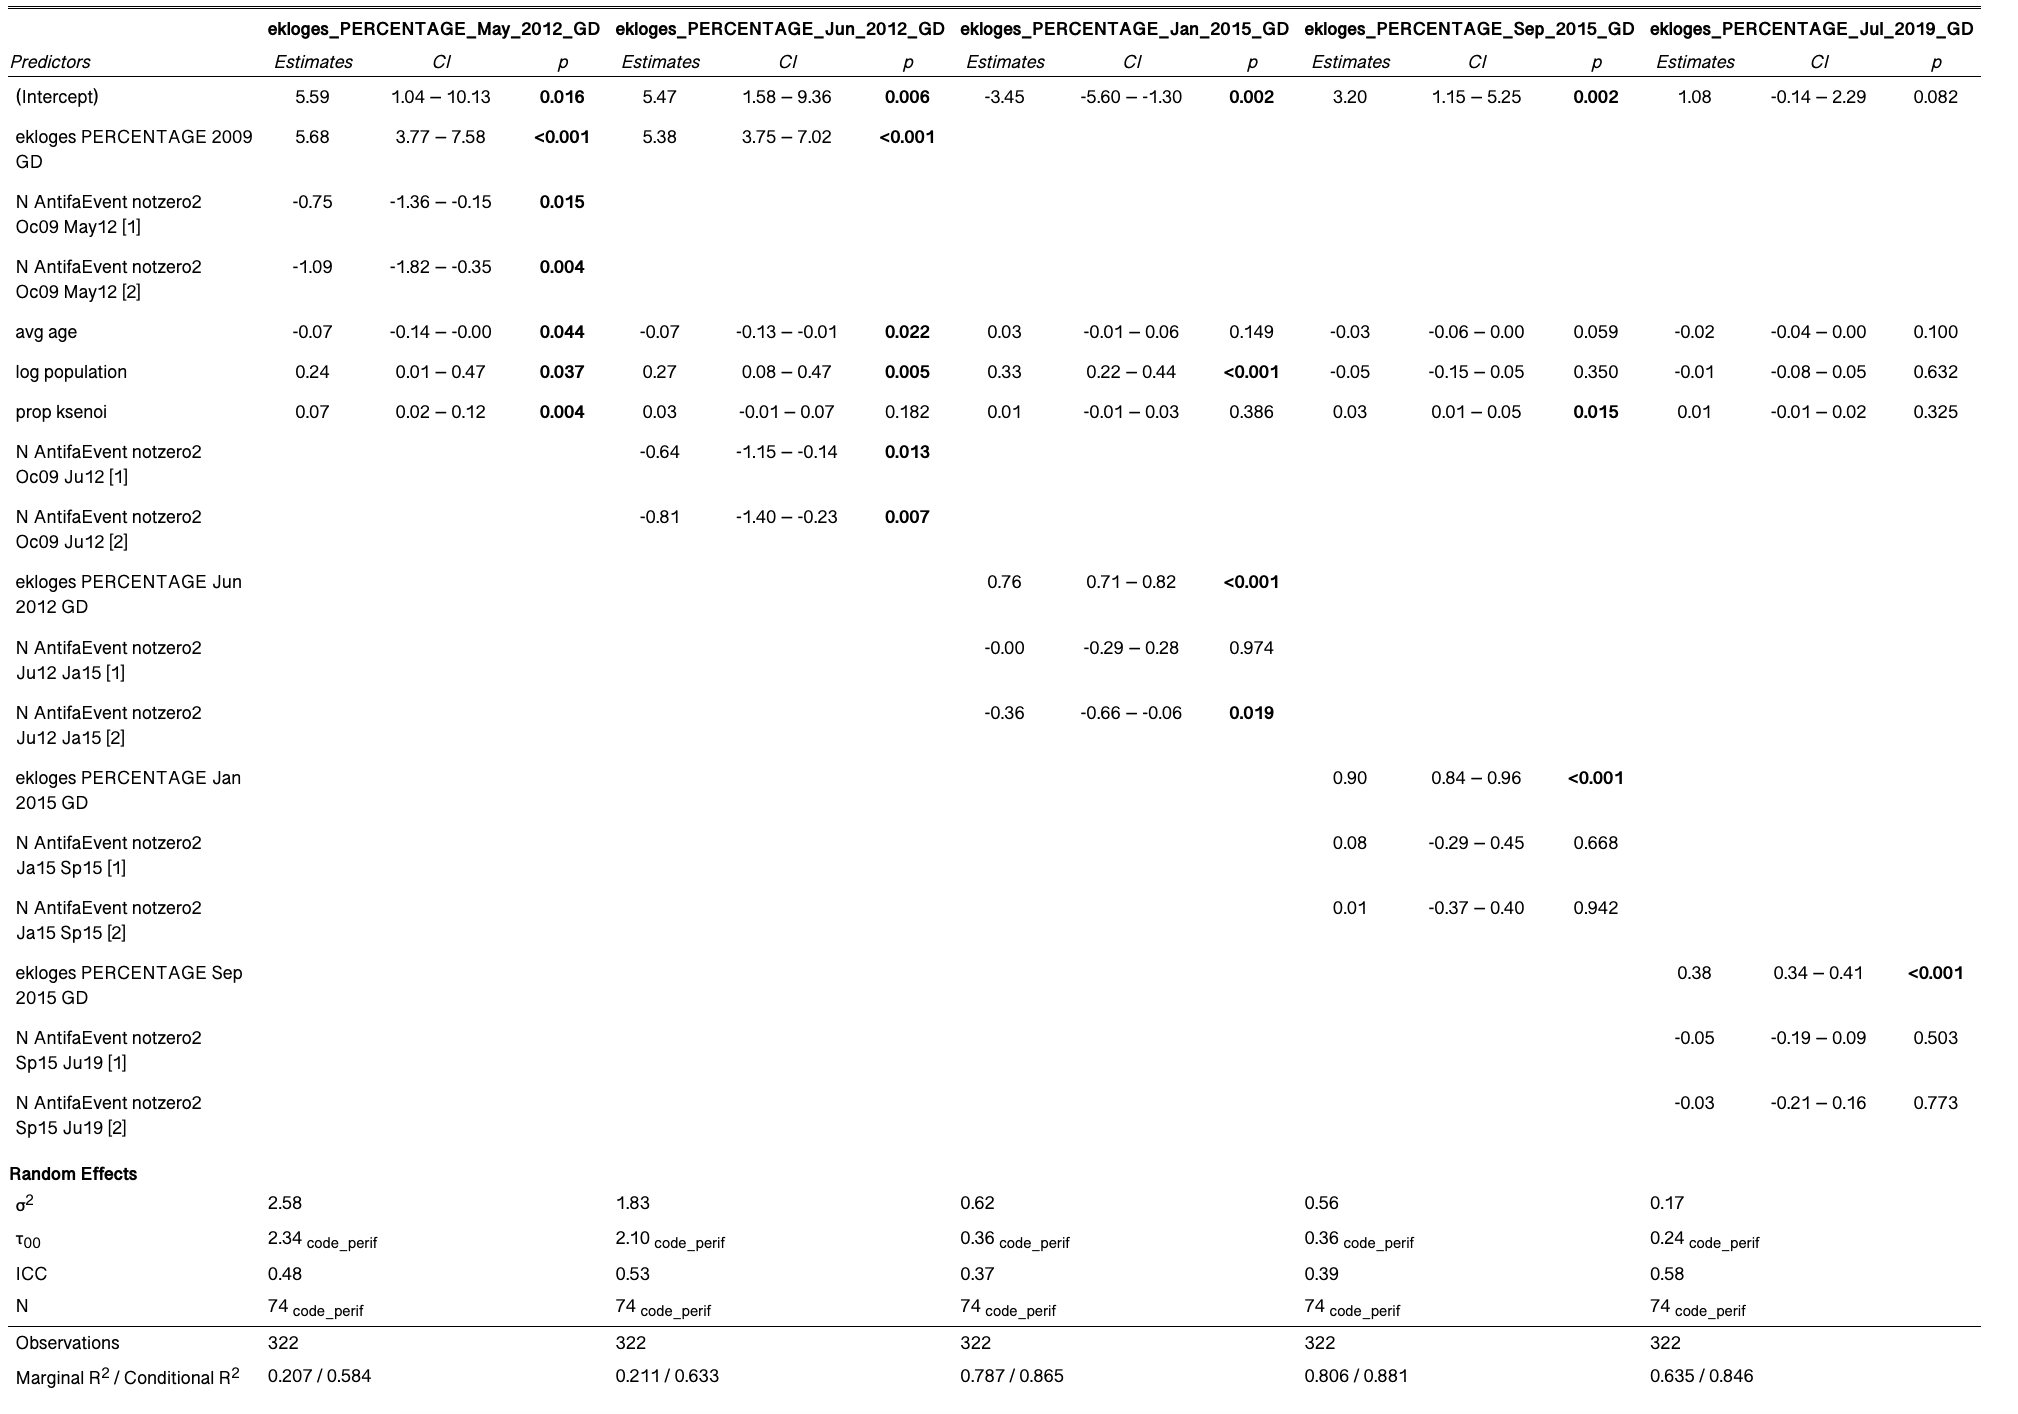
\includegraphics[width=0.99\textwidth]{Table_1.png}
    \end{itemize}
	\item
    Results (Original Table 1)
    \begin{itemize}
    \item 
	 Model 1: A linear mixed-effects model was built for each of the national elections from May 2012 onward.These results are not only statistically, but also practically, significant: with a national yield of around 7\% in the elections of May 2012, the impact of frequent anti-far right protests corresponds to a reduction of around one-sixth of the electoral power of GD.\\
	 
	Model 2: The effect of anti-far right protest is similar to that of Model 1: municipalities with protest events yield significantly lower results for the GD compared to the municipalities with no events. our analysis shows a direct relationship between social movement mobilization and electoral outcomes: protests against the far right took a toll on its electoral result.
     \end{itemize}
    \item
    My extension
    \begin{itemize}
    	\item
    	Extension idea: Fit linear regression model instead of mixed effects models.
     \end{itemize}
     \lstinputlisting[language=R, firstline=121, lastline=137]{R code Replication.R}
      \begin{itemize}
     	\item Results: It can be seen from the regression results that the coefficients of Model 1 and Model 2 are statistically significant, but the R square is small, indicating that the model fitting effect is not good.
     \end{itemize}
     	
\end{itemize}     

\begin{table}[!htbp] 
	\centering 
	\caption{Extension for Linear Regression Models } 
	\label{} 
	\small
	\renewcommand{\tabularxcolumn}[1]{m{#1}} 
	\begin{tabularx}{\textwidth}{@{\extracolsep{5pt}}l *{5}{X}@{}} 
		\hline 
		\hline 
		& \multicolumn{5}{c}{\textit{Dependent variable:}} \\ 
		\cline{2-6} 
		& May\_2012& Jun\_2012 & Jan\_2015 & Sep\_2015 & Jul\_2019\\ 
		& (1) & (2) & (3) & (4) & (5)\\ 
		\hline 
		ekloges\_PERCENTAGE\_2009\_GD & 7.746$^{***}$ & 7.017$^{***}$ &  &  &  \\ 
		& (0.986) & (0.879) &  &  &  \\ 
		N\_AntifaEvent\_notzero2\_Oc09\_May121 & $-$0.989$^{**}$ &  &  &  &  \\ 
		& (0.382) &  &  &  &  \\ 
		N\_AntifaEvent\_notzero2\_Oc09\_May122 & $-$1.315$^{***}$ &  &  &  &  \\ 
		& (0.458) &  &  &  &  \\ 
		N\_AntifaEvent\_notzero2\_Oc09\_Ju121 &  & $-$0.670$^{**}$ &  &  &  \\ 
		&  & (0.338) &  &  &  \\ 
		N\_AntifaEvent\_notzero2\_Oc09\_Ju122 &  & $-$1.208$^{***}$ &  &  &  \\ 
		&  & (0.387) &  &  &  \\ 
		ekloges\_PERCENTAGE\_Jun\_2012\_GD &  &  & 0.758$^{***}$ &  &  \\ 
		&  &  & (0.025) &  &  \\ 
		N\_AntifaEvent\_notzero2\_Ju12\_Ja151 &  &  & $-$0.017 &  &  \\ 
		&  &  & (0.168) &  &  \\ 
		N\_AntifaEvent\_notzero2\_Ju12\_Ja152 &  &  & $-$0.501$^{***}$ &  &  \\ 
		&  &  & (0.168) &  &  \\ 
		ekloges\_PERCENTAGE\_Jan\_2015\_GD &  &  &  & 0.950$^{***}$ &  \\ 
		&  &  &  & (0.028) &  \\ 
		N\_AntifaEvent\_notzero2\_Ja15\_Sp151 &  &  &  & 0.051 &  \\ 
		&  &  &  & (0.219) &  \\ 
		N\_AntifaEvent\_notzero2\_Ja15\_Sp152 &  &  &  & 0.237 &  \\ 
		&  &  &  & (0.218) &  \\ 
		ekloges\_PERCENTAGE\_Sep\_2015\_GD &  &  &  &  & 0.377$^{***}$ \\ 
		&  &  &  &  & (0.017) \\ 
		N\_AntifaEvent\_notzero2\_Sp15\_Ju191 &  &  &  &  & $-$0.044 \\ 
		&  &  &  &  & (0.094) \\ 
		N\_AntifaEvent\_notzero2\_Sp15\_Ju192 &  &  &  &  & $-$0.009 \\ 
		&  &  &  &  & (0.116) \\ 
		avg\_age & $-$0.010 & $-$0.015 & 0.030$^{*}$ & $-$0.032$^{**}$ & $-$0.051$^{***}$ \\ 
		& (0.038) & (0.034) & (0.017) & (0.016) & (0.011) \\ 
		log\_population & 0.415$^{***}$ & 0.449$^{***}$ & 0.385$^{***}$ & $-$0.213$^{***}$ & $-$0.046 \\ 
		& (0.120) & (0.107) & (0.057) & (0.053) & (0.035) \\ 
		prop\_ksenoi & 0.109$^{***}$ & 0.069$^{***}$ & $-$0.006 & 0.032$^{***}$ & $-$0.005 \\ 
		& (0.026) & (0.023) & (0.012) & (0.011) & (0.008) \\ 
		Constant & 0.480 & 0.824 & $-$4.009$^{***}$ & 4.413$^{***}$ & 2.991$^{***}$ \\ 
		& (2.384) & (2.122) & (1.052) & (1.025) & (0.669) \\ 
		\hline 
		Observations & 322 & 322 & 322 & 322 & 322 \\ 
		R$^{2}$ & 0.308 & 0.311 & 0.794 & 0.817 & 0.667 \\ 
		Adjusted R$^{2}$ & 0.295 & 0.298 & 0.790 & 0.813 & 0.660 \\ 
		Residual Std. Error (df = 315) & 2.192 & 1.958 & 0.976 & 0.952 & 0.619 \\ 
		F Statistic (df = 6; 315) & 23.407$^{***}$ & 23.673$^{***}$ & 201.749$^{***}$ & 233.657$^{***}$ & 104.944$^{***}$ \\ 
		\hline 
		\multicolumn{6}{p{\dimexpr\textwidth-2\tabcolsep-2\arrayrulewidth\relax}}{\textit{Note:} $^{*}p<0.1$; $^{**}p<0.05$; $^{***}p<0.01$. Standard errors in parentheses.}
	\end{tabularx} 
\end{table}

\section*{Second stage of study - Tango}
\vspace{.25cm}
\begin{itemize}
	\item
	Branching Research Question
	\begin{itemize}
		\item How do Tango events affect “electoral results of the GD?
	\end{itemize}
	\item
	Hypothesis
	\begin{itemize}
		\item H0: Tango events  do NOT affect“electoral results of the GD.\\
		H1: Tango events affect “electoral results of the GD.\\
	\end{itemize}
	\item
	Data
	\begin{itemize}
		\item 
		Variable description\\
		- Dependent variable: the main dependent variable (DV) is the electoral results of GD, measured as the percentage of votes received by the GD per municipality.\\
		- Independent variable:The main IV is a binary variable---Tango events (Yes 1or No 0)\\
		Tango events: events especially against for GD events
	\end{itemize}
	\item 
	Replication of codes and table 2
	\begin{itemize}
		\lstinputlisting[language=R, firstline=141, lastline=145]{R code Replication.R}
		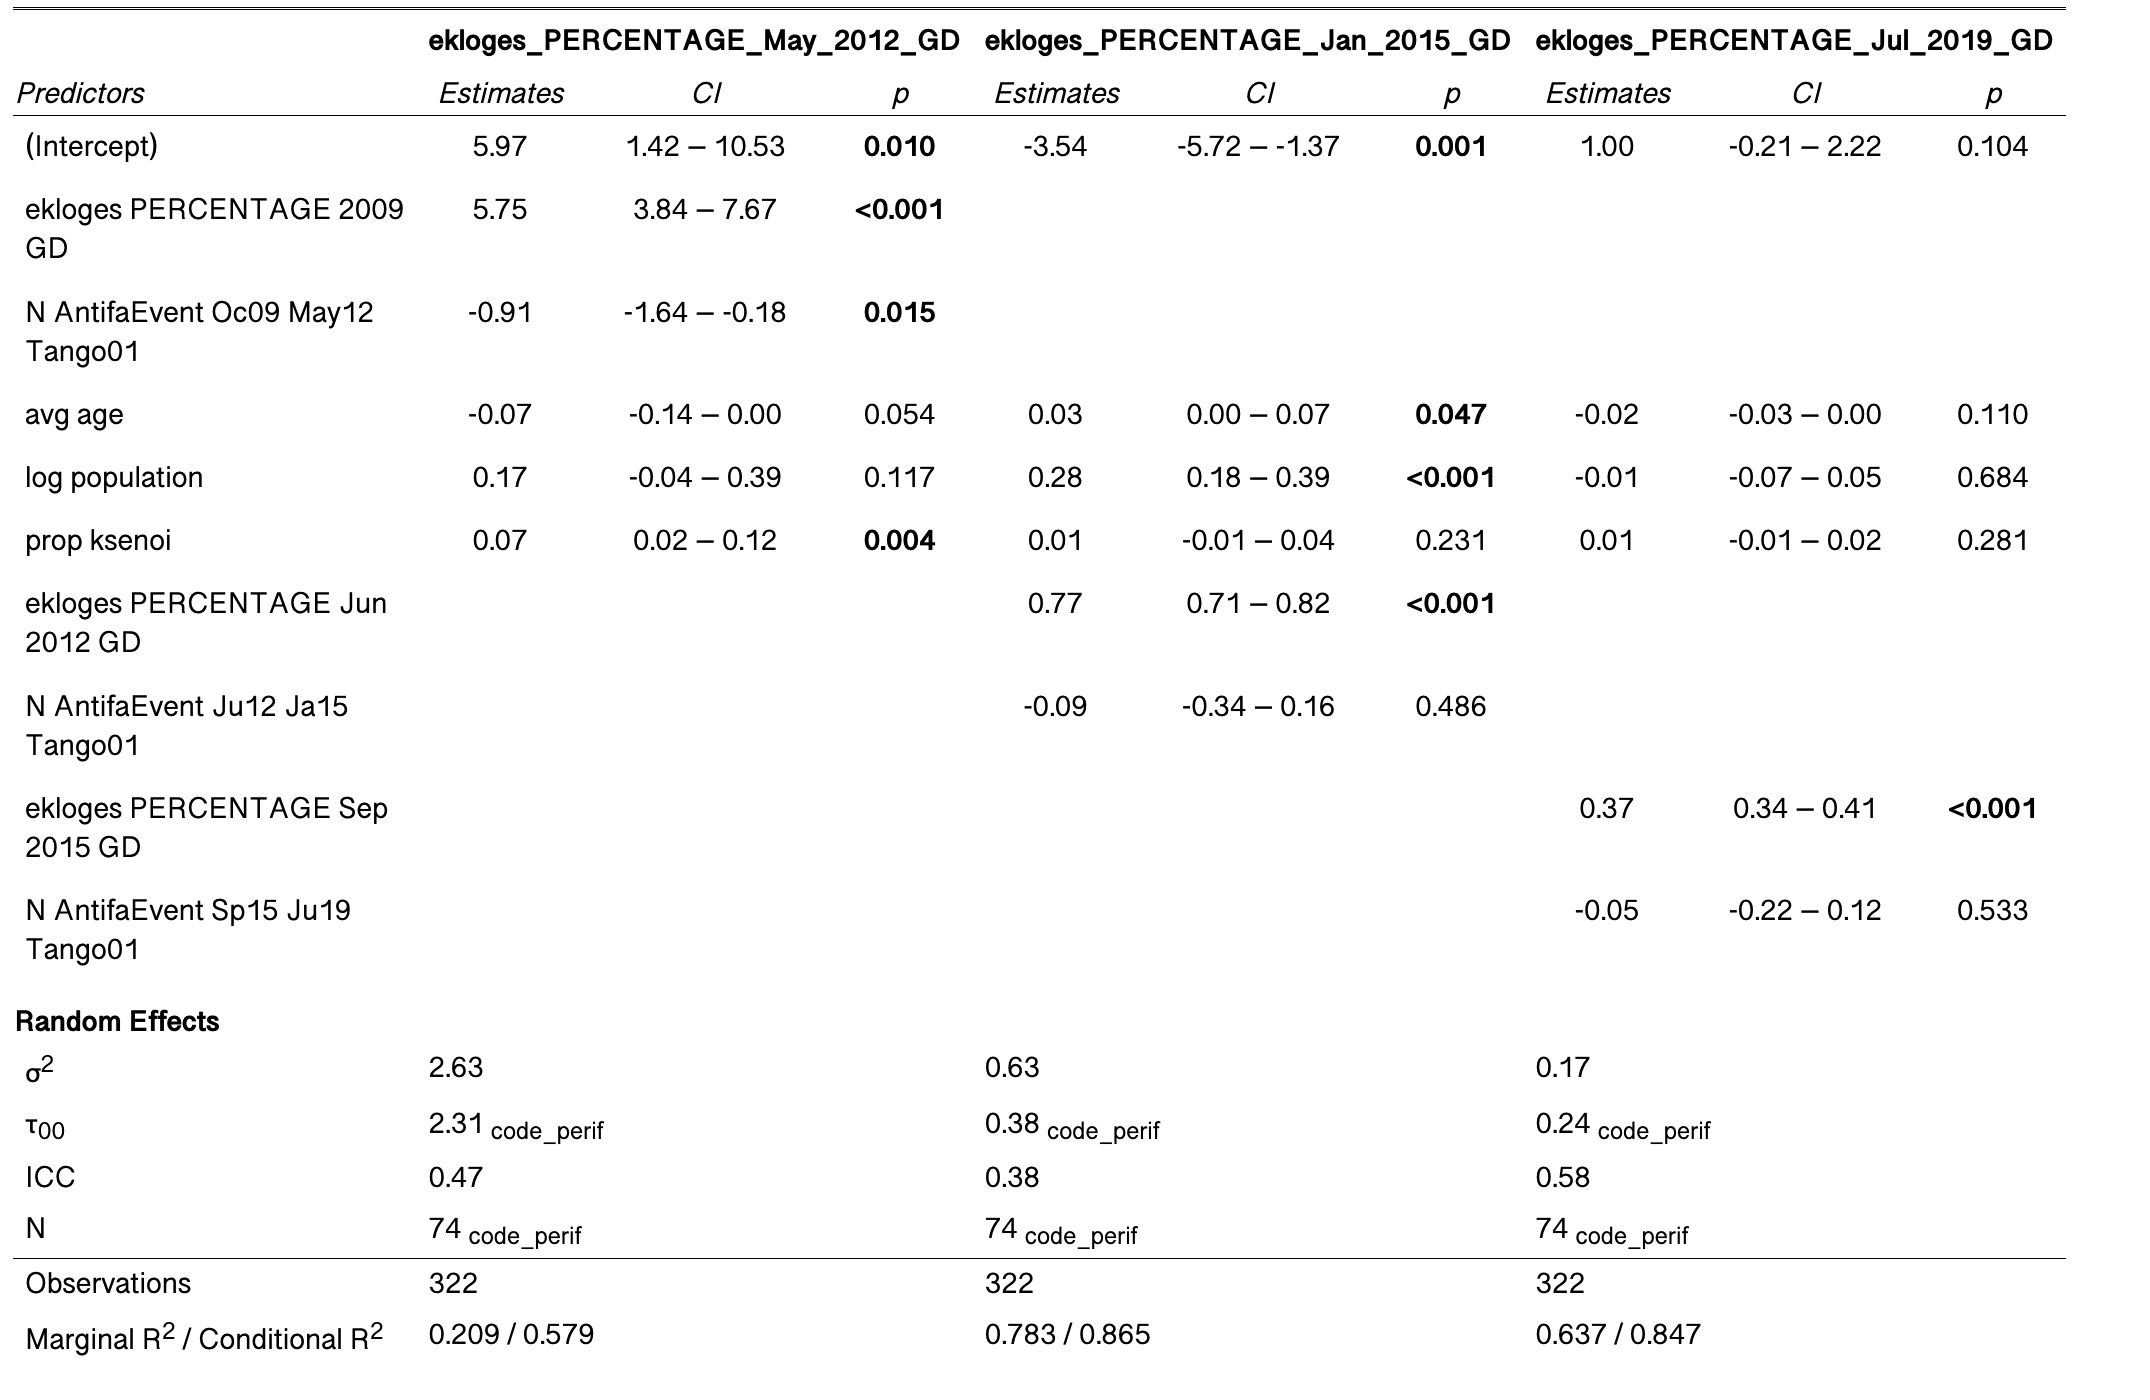
\includegraphics[width=0.99\textwidth]{Table_2.png}
	\end{itemize}
	\item
	Results  (Original Table 2)
	\begin{itemize}
		\item 
		The results  (Original Table 2) suggest that, for the elections of May 2012, municipalities with at least one tango event had much lower electoral outcomes for the GD compared to municipalities with no tango events.
	\end{itemize}
	\item
	My extension
	\begin{itemize}
		\item
		Extension idea: Fit linear regression model instead of mixed effects models.
	\end{itemize}
	\lstinputlisting[language=R, firstline=149, lastline=152]{R code Replication.R}
	\begin{itemize}
		\item Results: It can be seen from the regression results that the coefficients of Model 1  are statistically significant, but the R square is small, indicating that the model fitting effect is not good.
	\end{itemize}
	
\end{itemize}     

\begin{table}[!htbp] 
	\centering 
	\caption{Extension for Linear Regression Models } 
	\label{} 
	\small
	\begin{tabularx}{\textwidth}{@{\extracolsep{5pt}}l *{3}{D{.}{.}{-3}} @{}} 
		\hline 
		\hline \\[-1.8ex] 
		& \multicolumn{3}{c}{\textit{Dependent variable:}} \\ 
		\cline{2-4} 
		& \multicolumn{1}{c}{\textit{May\_2012}} & \multicolumn{1}{c}{\textit{Jan\_2015}} & \multicolumn{1}{c}{\textit{Jul\_2019}} \\ 
		& \multicolumn{1}{c}{(1)} & \multicolumn{1}{c}{(2)} & \multicolumn{1}{c}{(3)}\\ 
		\hline \\[-1.8ex] 
		ekloges\_PERCENTAGE\_2009\_GD & 7.518^{***} &  &  \\ 
		& (0.993) &  &  \\ 
		N\_AntifaEvent\_Oc09\_May12\_Tango01 & -1.307^{***} &  &  \\ 
		& (0.451) &  &  \\ 
		ekloges\_PERCENTAGE\_Jun\_2012\_GD &  & 0.759^{***} &  \\ 
		&  & (0.026) &  \\ 
		N\_AntifaEvent\_Ju12\_Ja15\_Tango01 &  & -0.160 &  \\ 
		&  & (0.146) &  \\ 
		ekloges\_PERCENTAGE\_Sep\_2015\_GD &  &  & 0.376^{***} \\ 
		&  &  & (0.017) \\ 
		N\_AntifaEvent\_Sp15\_Ju19\_Tango01 &  &  & -0.031 \\ 
		&  &  & (0.118) \\ 
		avg\_age & -0.007 & 0.040^{**} & -0.051^{***} \\ 
		& (0.038) & (0.017) & (0.010) \\ 
		log\_population & 0.340^{***} & 0.328^{***} & -0.045 \\ 
		& (0.114) & (0.054) & (0.033) \\ 
		prop\_ksenoi & 0.110^{***} & -0.002 & -0.004 \\ 
		& (0.026) & (0.012) & (0.007) \\ 
		Constant & 0.970 & -4.044^{***} & 2.949^{***} \\ 
		& (2.378) & (1.075) & (0.666) \\ 
		\hline \\[-1.8ex] 
		Observations & \multicolumn{1}{c}{322} & \multicolumn{1}{c}{322} & \multicolumn{1}{c}{322} \\ 
		R$^{2}$ & \multicolumn{1}{c}{0.301} & \multicolumn{1}{c}{0.787} & \multicolumn{1}{c}{0.666} \\ 
		Adjusted R$^{2}$ & \multicolumn{1}{c}{0.290} & \multicolumn{1}{c}{0.784} & \multicolumn{1}{c}{0.661} \\ 
		Residual Std. Error (df = 316) & \multicolumn{1}{c}{2.200} & \multicolumn{1}{c}{0.990} & \multicolumn{1}{c}{0.618} \\ 
		F Statistic (df = 5; 316) & \multicolumn{1}{c}{27.246$^{***}$} & \multicolumn{1}{c}{233.736$^{***}$} & \multicolumn{1}{c}{126.228$^{***}$} \\ 
		\hline 
		\hline \\[-1.8ex] 
		\multicolumn{4}{l}{\textit{Note:} $^{*}$p$<$0.1; $^{**}$p$<$0.05; $^{***}$p$<$0.01} \\ 
	\end{tabularx} 
\end{table}

\section*{Second stage of study - Timing}
\vspace{.25cm}
\begin{itemize}
	\item
	Branching Research Question
	\begin{itemize}
		\item How does Timing of protest events affect electoral results of the GD?
	\end{itemize}
	\item
	Hypothesis
	\begin{itemize}
		\item H0: Timing of protest  events does NOT affect electoral results of the GD.\\
		H1: Timing of protest events affects electoral results of the GD.\\
	\end{itemize}
	\item
	Data
	\begin{itemize}
		\item 
		Variable description\\
		- Dependent variable: the main dependent variable (DV) is the electoral results of GD, measured as the percentage of votes received by the GD per municipality.\\
		- Independent variable:The main IV is a categorical variable describing the temporal proximity to the parliamentary election.\\
	\end{itemize}
	\item 
	Replication of codes and table 3
	\begin{itemize}
		\lstinputlisting[language=R, firstline=167, lastline=171]{R code Replication.R}
		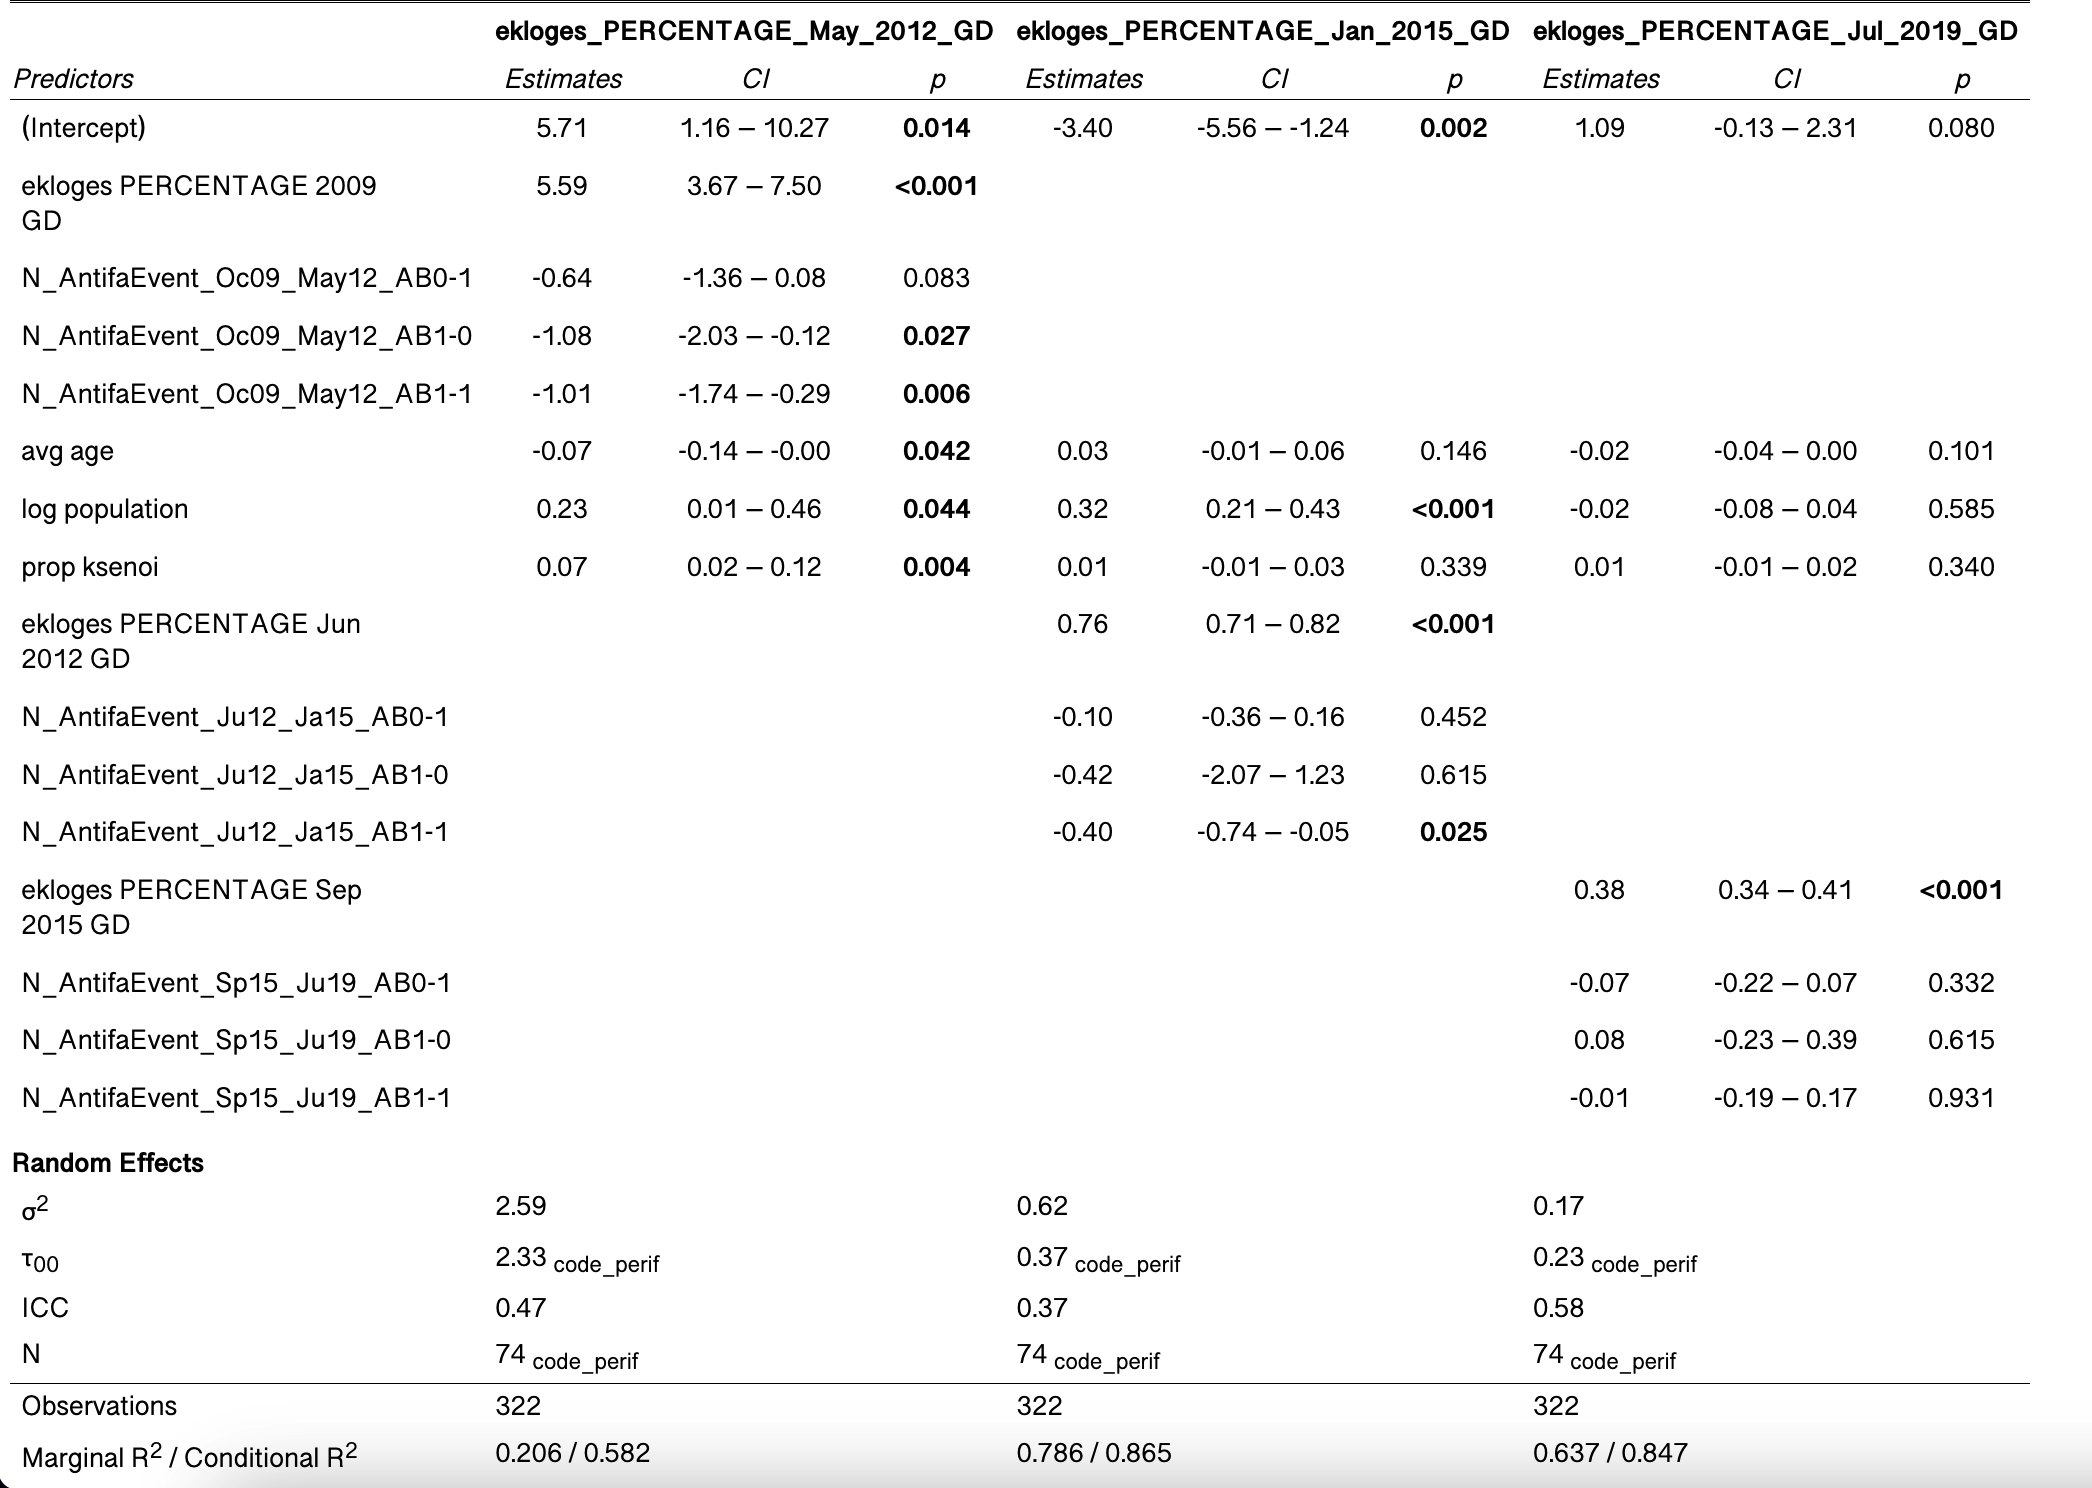
\includegraphics[width=0.99\textwidth]{Table_3.png}
	\end{itemize}
	\item
	Results  (Original Table 3)
	\begin{itemize}
		\item 
		The results (see Original Table 3) for May 2012 suggest that organizing at least one proximate protest event against the far right, compared to organizing no events at all, corresponds to a smaller electoral outcome for the GD, similar in magnitude to that identified by previous models which was around one-sixth of the 7\% of the national vote.
		
		The evidence presented shows that the synchronization of protest and electoral cycles makes protest more effective: protests against the far right taking place right before the next election are much more effective than those temporally more distant.
	\end{itemize}
	\item
	My extension
	\begin{itemize}
		\item
		Extension idea: Fit linear regression model instead of mixed effects models.
	\end{itemize}
	\lstinputlisting[language=R, firstline=176, lastline=178]{R code Replication.R}
	\begin{itemize}
		\item Results: It can be seen from the regression results that the all of the coefficients of Models are not statistically significant.
	\end{itemize}
	
\end{itemize}    

\begin{table}[!htbp] 
	\centering 
	\caption{Extension for Linear Regression Models} 
	\label{} 
	\setlength{\tabcolsep}{3pt}
	\tiny
	\begin{tabular}{@{\extracolsep{5pt}}lccc} 
		\\[-1.8ex]\hline 
		\hline \\[-1.8ex] 
		& \multicolumn{3}{c}{\textit{Dependent variable:}} \\ 
		\cline{2-4} 
		\\[-1.8ex] & \multicolumn{1}{c}{May\_2012} & \multicolumn{1}{c}{Jan\_2015} & \multicolumn{1}{c}{Jul\_2019} \\ 
		\\[-1.8ex] & \multicolumn{1}{c}{(1)} & \multicolumn{1}{c}{(2)} & \multicolumn{1}{c}{(3)}\\ 
		\hline \\[-1.8ex] 
		ekloges\_PERCENTAGE\_2009\_GD & 7.645$^{***}$ &  &  \\ 
		& (0.992) &  &  \\ 
		& & & \\ 
		N\_AntifaEvent\_Oc09\_May12\_AB0-1 & -0.677 &  &  \\ 
		& (0.464) &  &  \\ 
		& & & \\ 
		N\_AntifaEvent\_Oc09\_May12\_AB1-0 & -1.591$^{***}$ &  &  \\ 
		& (0.577) &  &  \\ 
		& & & \\ 
		N\_AntifaEvent\_Oc09\_May12\_AB1-1 & -1.244$^{***}$ &  &  \\ 
		& (0.454) &  &  \\ 
		& & & \\ 
		ekloges\_PERCENTAGE\_Jun\_2012\_GD &  & 0.754$^{***}$ &  \\ 
		&  & (0.026) &  \\ 
		& & & \\ 
		N\_AntifaEvent\_Ju12\_Ja15\_AB0-1 &  & -0.168 &  \\ 
		&  & (0.152) &  \\ 
		& & & \\ 
		N\_AntifaEvent\_Ju12\_Ja15\_AB1-0 &  & -0.731 &  \\ 
		&  & (0.988) &  \\ 
		& & & \\ 
		N\_AntifaEvent\_Ju12\_Ja15\_AB1-1 &  & -0.503$^{**}$ &  \\ 
		&  & (0.197) &  \\ 
		& & & \\ 
		ekloges\_PERCENTAGE\_Sep\_2015\_GD &  &  & 0.379$^{***}$ \\ 
		&  &  & (0.017) \\ 
		& & & \\ 
		N\_AntifaEvent\_Sp15\_Ju19\_AB0-1 &  &  & -0.072 \\ 
		&  &  & (0.096) \\ 
		& & & \\ 
		N\_AntifaEvent\_Sp15\_Ju19\_AB1-0 &  &  & 0.019 \\ 
		&  &  & (0.219) \\ 
		& & & \\ 
		N\_AntifaEvent\_Sp15\_Ju19\_AB1-1 &  &  & 0.043 \\ 
		&  &  & (0.119) \\ 
		& & & \\ 
		avg\_age & -0.009 & 0.032$^{*}$ & -0.051$^{***}$ \\ 
		& (0.038) & (0.017) & (0.011) \\ 
		& & & \\ 
		log\_population & 0.409$^{***}$ & 0.375$^{***}$ & -0.052 \\ 
		& (0.120) & (0.058) & (0.035) \\ 
		& & & \\ 
		prop\_ksenoi & 0.110$^{***}$ & -0.005 & -0.005 \\ 
		& (0.026) & (0.012) & (0.008) \\ 
		& & & \\ 
		Constant & 0.545 & -3.992$^{***}$ & 2.997$^{***}$ \\ 
		& (2.379) & (1.061) & (0.670) \\ 
		& & & \\ 
		\hline \\[-1.8ex] 
		Observations & \multicolumn{1}{c}{322} & \multicolumn{1}{c}{322} & \multicolumn{1}{c}{322} \\ 
		R$^{2}$ & \multicolumn{1}{c}{0.312} & \multicolumn{1}{c}{0.791} & \multicolumn{1}{c}{0.668} \\ 
		Adjusted R$^{2}$ & \multicolumn{1}{c}{0.296} & \multicolumn{1}{c}{0.786} & \multicolumn{1}{c}{0.660} \\ 
		Residual Std. Error (df = 314) & \multicolumn{1}{c}{2.191} & \multicolumn{1}{c}{0.984} & \multicolumn{1}{c}{0.619} \\ 
		F Statistic (df = 7; 314) & \multicolumn{1}{c}{20.322$^{***}$} & \multicolumn{1}{c}{169.783$^{***}$} & \multicolumn{1}{c}{90.067$^{***}$} \\ 
		\hline 
		\hline \\[-1.8ex] 
		\textit{Note:}  & \multicolumn{3}{r}{$^{*}$p$<$0.1; $^{**}$p$<$0.05; $^{***}$p$<$0.01} \\ 
	\end{tabular} 
\end{table}



\end{document}
